\documentclass[a4paper, 11pt]{report}
\usepackage{epsfig}
\usepackage{graphics}
\usepackage{multirow}
\usepackage{multicol}
\usepackage{fancyhdr}
\usepackage{lastpage}
\usepackage{latexsym}
\usepackage[hang, scriptsize, bf]{caption}

\usepackage[utf8]{inputenc}

\usepackage{enumerate}

\usepackage{tikz}
\usepackage[european]{circuitikz}

\usepackage{stackengine}
\usepackage{scalerel}
\usepackage{xcolor}
\newcommand\dangersign[1][2ex]{%
  \renewcommand\stacktype{L}%
  \scaleto{\stackon[1.3pt]{\color{red}$\triangle$}{\tiny\bfseries !}}{#1}%
}
%-------------------------------------------------------------------------------

\textwidth      170mm
\textheight     240mm
\hoffset        -10mm 
\voffset        -10mm
\oddsidemargin   5mm
\evensidemargin -5mm
\topmargin	    -5mm

%-------------------------------------------------------------------------------


\newcommand{\eduTitle}{Zadání laboratoře}
\newcommand{\eduID}{5}
\newcommand{\eduTopic}{Integrovaný obvod a logická hradla}
\newcommand{\eduDetails}{
\footnotesize
Cíle: 
Seznámit se s významem logických úrovní/hodnot (log.0, log.1)
v dané realizaci
a
s konkrétním IO (integrovaným obvodem),
prakticky ověřit funkčnost hradel z IO 
a 
využít hradla z IO ke konstrukci vybraných praktických obvodů. 
}
%
\newcommand{\subjIDlong}{Elektronika pro informační technologie}
\newcommand{\schoolDlong}{Vysoké učení technické v Brně}
\newcommand{\schoolDshort}{VUT v Brně}
\newcommand{\facultylDlong}{Fakulta informačních technologií}
\newcommand{\facultylDshort}{FIT}
%
\newcommand{\subjIDshort}{IEL}
%
\newcommand{\actYear}{2024}
\newcommand{\acadYear}{2024/2025}

\usepackage[hidelinks]{hyperref}

\renewcommand{\figurename}{Obrázek}
\renewcommand{\tablename}{Tabulka}

%-------------------------------------------------------------------------------

\newcommand*\circled[1]{\tikz[baseline=(char.base)]{
            \node[shape=circle,draw,inner sep=2pt] (char) {#1};}}

%-------------------------------------------------------------------------------

\newcounter{cntInfo}
\newcommand{\info}[3]{\refstepcounter{cntInfo}
\paragraph*{
\circled{\thecntInfo}~{\sc \fbox{#1}} {\sc #2}  
} 
\paragraph{\textmd{#3}} }


\newcommand\encircle[1]{%
  \tikz[baseline=(X.base)] 
    \node (X) [draw, shape=circle, fill=yellow, inner sep=0] {\strut #1};}

%-------------------------------------------------------------------------------

\begin{document}

%-------------------------------------------------------------------------------

\pagestyle{fancy}
\renewcommand{\headrulewidth}{0pt}
\renewcommand{\theenumi}{\Alph{enumi}}  
\lhead{}
\chead{}
\rhead{}
\lfoot{\centering
\tiny \itshape \eduTitle ~č. \eduID \hspace{0.1mm} z předmětu \subjIDshort \hspace{1mm} 
(ak. r. \acadYear). \copyright~\actYear~Josef~Strnadel,~\facultylDshort~\schoolDshort. Připomínky zasílejte na \href{mailto:strnadel@fit.vut.cz}{strnadel@fit.vut.cz}\\ 
Časové razítko PDF dokumentu [\pdfcreationdate]. 
Sazba byla provedena systémem \LaTeX.
 }
\cfoot{}
%-------------------------------------------------------------------------------

%-------------------------------------------------------------------------------

\begin{center}
\scalebox{0.1}{
\includegraphics{FIT_cernobile_CZ.pdf}}
\parbox{120mm}{
\textsc{\footnotesize\schoolDlong}, 
\textsc{\footnotesize\facultylDlong}\\
}
{
\Large
\textsc{\subjIDlong} (\textsc{\subjIDshort}), \textsc{ak. r. \acadYear}}

\hrulefill

\vspace{4mm}
\parbox{\linewidth}{
\centering
%
{\Huge \textsc{\eduTitle~č.~\fbox{\eduID}}}\\
{\textsc{,,\eduTopic''}}\\

}

\end{center}

{\it \eduDetails}

\hrulefill

%-------------------------------------------------------------------------------
\info{Motivace}{aneb ,,Proč tomu věnovat čas a jaké kompetence lze získat ?''}{
Na základě sady experimentů budete moci ověřit, pochopit a objasnit 
význam vývodů konkrétního IO a logických úrovní/hodnot, 
činnost NAND hradla dané realizace a 
jeho vybraných aplikací.
}

%-------------------------------------------------------------------------------
\info{Výstup a způsob jeho hodnocení}{aneb ,,Co se ode mne očekává a co za to ?''}{
Za záznam výsledků měření do tabulky, předvedení a objasnění činnosti bistabilního klopného obvodu (KO)
a
za ověření a objasnění činnosti astabilního popř. monostabilního KO
lze získat až {\bf 3 body}.
}

%-------------------------------------------------------------------------------
\info{Prostředky}{aneb ,,Co je k dispozici ?''\vspace{-4mm}}{
~
}

\hspace{-8mm}
\parbox{15mm}{
\vspace{2mm}
\dangersign[8ex] 
}
\parbox{155mm}{
Zdroj ss. napětí s omezením proudu,
nepájivé pole, 
krabička s konstrukčními prvky (rezistory, diody, kondenzátory, tlačítko, IO s NAND hradly, vodiče), 
měřicí přístroje. 
\it
\textcolor{red}{
\hspace{28mm}Integrovaný obvod (IO) nevyjímejte z nepájivého pole! 
}
}
\\

\vspace{-2mm}

%-------------------------------------------------------------------------------
\info{Základní schéma(ta)}{aneb ,,Z čeho se bude vycházet ?''}{
~
}

\vspace{-10mm}

\begin{figure}[h]
  \begin{center}

\hspace{-4mm}
\parbox{40mm}{
\flushleft
\scalebox{.95}{
    \begin{circuitikz}  
        \draw (0,0) node[ieeestd nand port] (nand1) {};
%      
        \node at (nand1.in 1) [left] {$x$};
        \node at (nand1.in 2) [left] {$y$};
        \node at (nand1.out) [right] {$\overline{x \wedge y}$};

        \ctikzset{tripoles/european not symbol=ieee circle};
        \draw (.75,-1.5) node[nand port] (nand2) {};
%
        \node at (nand2.in 1) [left] {$x$};
        \node at (nand2.in 2) [left] {$y$};
        \node at (nand2.out) [right] {$\overline{x \wedge y}$};

        \node at (nand1.out) [left=27mm] {a)};
        \node at (nand2.out) [left=25mm] {b)};
   \end{circuitikz}
}
\vspace{0mm}    
}
\hspace{16mm}
\footnotesize
c)
\parbox{30mm}{
\rotatebox{00}{
\scalebox{.3}{
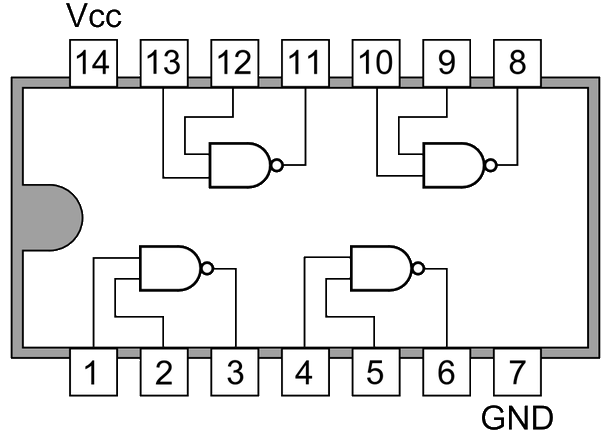
\includegraphics[trim={0mm 0mm 0mm 0mm},clip]{7400us.png}
}}}
\\[+4mm]

\footnotesize
\parbox{200mm}{
d)
\centering
\scalebox{1.05}{
\begin{tabular}{|c|c|c||c|}
\hline
\multicolumn{2}{|c|}{\bf Vstupy} & \bf Výstup & \parbox{75mm}{\centering {\bf Napěťové úrovně} pro log.0/1 \\na v(ý)stupech
TTL logických hradel} \\[10pt]
\hline
\parbox{2mm}{\vspace{3mm}$x$} & \parbox{2mm}{\vspace{3mm}$y$} & \parbox{8mm}{\vspace{3mm}$\overline{x \wedge y}$} & \multirow{5}{*}{
\scalebox{.4}{
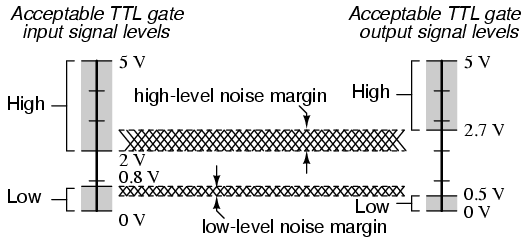
\includegraphics[trim={0mm 0mm 0mm 0mm},clip]{ttl_levels.png}
}
} \\[24pt]
\cline{1-3}
log.{\bf 0} & log.{\bf 0}& log.{\bf 1}&\\[5pt]
\cline{1-3}
log.{\bf 0} & log.{\bf 1}& log.{\bf 1}&\\[5pt]
\cline{1-3}
log.{\bf 1} & log.{\bf 0}& log.{\bf 1}&\\[5pt]
\cline{1-3}
log.{\bf 1} & log.{\bf 1}& log.{\bf 0}&\\[5pt]
\hline
\end{tabular}
}
}

\vspace{0mm}
   \caption{Varianty schematické značky 2vstup. hradla NAND (a, b), vývody a rozmístění hradel v IO s NAND hradly (c), očekávané vlastnosti 2vstupového hradla realizovaného v TTL logice (d)}
   \label{fig_io1}
  \end{center}
\vspace{-16mm}
\end{figure}


\newpage
%-------------------------------------------------------------------------------
\info{Postup samostatných činností}{aneb ,,Co dělat a na co si dát pozor ?''}{
~
}

\vspace{-8mm}
\begin{figure}[h]
  \begin{center}

\hspace{4mm}
 \scalebox{.65}{
      \begin{circuitikz}  
        \draw (0,0) node[ieeestd nand port] (nand1) {$G_R$};
        \draw (0,3) node[ieeestd nand port] (nand2) {$G_S$};

	\draw (nand1.in 2) to[short, -o] ++(-2.5,0) node[left] {$\overline{R}$} (nand1.in 2);
	\draw (nand2.in 1) to[short, -o] ++(-2.5,0) node[left] {$\overline{S}$} (nand2.in 1);
	
	\draw[short, *-, color=red] (-2,3.275)
	to[R, /tikz/circuitikz/bipoles/length=25pt, color=red, name=r1, l=\textcolor{red}{$R_1$}] (-2,1.5)
	to[R, /tikz/circuitikz/bipoles/length=25pt,  color=red, name=r2, l=\textcolor{red}{$R_2$}] (-2, -0.25)
	to[short, -*, color=red] (-2, -0.275);
	
	\draw[color=red] (r1.east) to (r2.west);
	\draw[color=red] (-2,1.5) to[short, -o] (-1.75,1.5) node[right] {\textcolor{red}{$+5~V$}};
	
        \draw (-3.8,1.25) node[ground, red, name=gnd] {}; 
        \draw (-3.5,1.5) node[cute spdt mid arrow, color=red, name=sw1] {\hspace{4mm}{$T$}};
	
	\draw[red] (-3.8,1.25) -- (-3.8,1.45);
	\draw[color=red] (sw1.out 1) to[short, -*, color=red] (-3.15,3.275);
	\draw[color=red] (sw1.out 2) to[short, -*, color=red] (-3.15,-.275);
	
	\node at (1.5, 0) (qn) {};
	\node at (1.5, 3) (q) {};

	\draw (1.5, 0) to[short, *-] (1.5, .5) node(q1) {};	
	\draw (1.5, 3) to[short, *-] (1.5, 2.5) node(qn1) {};	

	\draw (nand1.in 1) to[short] ++(0,.5) (nand1.in 1) node(r1) {};
	\draw (nand2.in 2) to[short] ++(0,-.5) (nand2.in 2) node(r2) {};

	\draw (q1) ++(0,0) -- (-1.075,2.225);
	\draw (qn1) ++(0,0) -- (-1.075,0.775);
	
	\draw (nand1.out) to[short, -o] ++(1,0) node[right] {$\overline{Q}$} (nand1.out) node[below] {\textcolor{blue}{\encircle{2}}};
	\draw (nand2.out) to[short, -o] ++(1,0) node[right] {$Q$} (nand2.out) node[above] {\textcolor{blue}{\encircle{1}}};

   \end{circuitikz}
   }
  \hspace{2mm}
 \scalebox{.65}{
      \begin{circuitikz}  
        \draw (0,0) node[ieeestd nand port] (nand1) {$G_1$};
        \draw (3,0) node[ieeestd nand port, rotate=180] (nand2) {\rotatebox{180}{$G_2$}};

       
        \draw (nand1.out) to (2,1.5) to [eC, name=c2, l=$C_2$] (4,1.5) {}; 
        \draw (nand2.out) to (1.0,1.5) to [eC, name=c1, l_=$C_1$] (-1.0,1.5) {}; 

        \draw (1.5,-1.75) node[ground, name=gnd] {}; 
\node at (gnd) {$\bullet$};
        
        \draw (nand1.in 1) to[short, *-*] (nand1.in 2)
        to[short] (-1.0825,-1.75)        
        to[R, l^=$R_1$, name=r1] (gnd)
        ;
        \draw (nand2.in 2) to[short, *-*] (nand2.in 1)
        to[short] (4.0825,-1.75)        
        to[R, l_=$R_2$, name=r2] (gnd)
        ;

        
	\draw (c1.east) -- (-1.0825,1.5) -- (nand1.in 1);
	\draw (c2.east) -- (4.0825,1.5) -- (nand2.in 1);

\ctikzset{bipoles/diode/height=0.25, bipoles/diode/width=0.25,}
	\draw (nand1.out) 
	to[short, *-, color=red] ++(0,0) (nand1.out) node[above=1mm] {\hspace{-3mm}\textcolor{blue}{\encircle{1}}}  
	to[led, color=red] (1.1,-0.75)  
	to[/tikz/circuitikz/bipoles/length=20pt, R, color=red] (1.1,-1.75)
	to[short, -*, color=red] ++(0,0);

	\draw (nand2.out) 
	to[short, *-, color=red] ++(0,0) (nand2.out) node[above=1mm] {\hspace{3mm}\textcolor{blue}{\encircle{2}}}  
	to[led, color=red] (1.95,-0.75) 
	to[/tikz/circuitikz/bipoles/length=20pt, R, color=red] (1.95,-1.75)
	to[short, -*, color=red] ++(0,0);
   \end{circuitikz}
   }
\hspace{2mm}
 \scalebox{.65}{
      \begin{circuitikz}  
        \draw (5,0) node[ieeestd nand port] (nandB) {$G_B$};
        \draw (0,0) node[ieeestd nand port] (nandA) {$G_A$};

	 \draw (nandB.in 1) to[short] (nandB.in 2);
	 \draw (nandB.out) 
	 to[short, -*] (6.5,0) 
	 to[short] (6.5,1.25) 
	 to[short] (-1.5,1.25) 
	 to[short] (-1.5,.28) 
	 to[short] (nandA.in 1) 
	 ;

	 \draw (nandB.out) to[short, -o] ++(1.25,0) (nandB.out)         
	 node[above] {\hspace{16mm}\textcolor{blue}{\encircle{2}}}
       ;
	 
	 \draw (nandA.in 2) to[short, -o] ++(-2,0) (nandA.in 2);

        \draw(nandA.out)  
        to[eC, l=$C$] (2.5,0) 
        to[short,-*] (3,0) node(rc) {} 
        node[above] {\textcolor{blue}{\encircle{1}}}
        to[short, -*] (3.925,0);
        \draw(rc) ++(0,0) 
        to[R, l=$R_T$] (3, -2) 
        to[short, -*] (3,-2.0)
        to[short] (-2.25,-2)
	to[push button, l=$T$] (-2.25,-.5)
	to[short, -*] (-2.25,-.275)
	to[R, l=$R_1$] (-2.25, 1.5) node[left] {$+5~V$}
	to[short, -o] (-2.25,1.75)
        ;
        
        \draw (3,-2) node[ground, name=gnd] {}; 



   \end{circuitikz}
   }
   

\vspace{-4mm}
\scriptsize
\hspace{-65mm}a) 
\hspace{45mm} b)  
\hspace{40mm} c)  

\vspace{-2mm}
   \caption{Schémata klopných obvodů (KO) k zapojení (volitelné části jsou zbarveny červeně): a) bistabilní KO typu RS, b)~astabilní KO, c) monostabilní KO; \parbox{4mm}{\vspace{-0mm}\scalebox{.75}{\protect\encircle{1}}}, \parbox{4mm}{\vspace{-0mm}\scalebox{.75}{\protect\encircle{2}}} jsou uzly, jejichž sledování by mělo přispět k objasněn dějů v obvodech}
   \label{fig_io2}
  \end{center}
  
\vspace{-12mm}  
\end{figure}

\begin{enumerate}[\bf {Experiment} 1:]

\item 
\begin{enumerate}[i)]
\item
{\bf Prostudujte} rozmístění vývodů IO (viz Obr. \ref{fig_io1}c) 
a 
{\bf připojte} na IO napájecí napětí, tj. 7. vývod IO k 0 V (GND) a 14. vývod IO k +5 V (Vcc). 

\item 
\parbox{125mm}{
S využitím tab. z Obr. \ref{fig_io1}c {\bf identifikujte} v IO alespoň dvě funkční NAND hradla.
\textcolor{red}{
\it Funkčnost hradla je nutno ověřit pro každou vstupní kombinaci !!!}
}
\parbox{5mm}{
\dangersign[5ex]\par
} 

\item
Z funkčních NAND hradel 
{\bf zapojte} obvod dle Obr. \ref{fig_io2}a a analyzujte jeho chování
pro kombinace předepsané v  
Tab. \ref{tab1}.
{\bf Odměřte} log. hodnoty a hodnoty napětí chybějící v Tab. \ref{tab1}, 
{\bf předveďte} a {\bf objasněte} činnost obvodu vyučující(mu).



\end{enumerate}

\vspace{-1mm}
\begin{table}[h]
\centering
\scalebox{0.75}{
\begin{tabular}{|c|c||c|c|c||c|}
\hline
\multicolumn{2}{|c||}{\bf vstupy} & \multicolumn{3}{|c||}{\bf výstupy/stav} & \multirow{3}{*}{\bf komentář} \\
\cline{1-5}
\multirow{1}{*}{\parbox{4mm}{\centering \vspace{1mm} $\overline{S}_t$}} & 
\multirow{1}{*}{\parbox{2mm}{\centering \vspace{1mm} $\overline{R}_t$}}   &  
$Q_{t}$  &
\multicolumn{2}{|c||}{$Q_{t+1}$}
&
\\[0pt]
\cline{1-5}
\multicolumn{4}{|c|}{[logická hodnota]} &  [V] &\\
\hline
\hline
\bf 0&\bf 1&X&&&$S_t=1$ při $R_t=0$ (``Set''): \textbf{zapiš} log.\textbf{1} ($Q_{t+1}$ = log.1)\\
\hline
\bf 1&\bf 0&X&&&$R_t=1$ při $S_t=0$ (``Reset''): \textbf{zapiš} log.\textbf{0} ($Q_{t+1}$ = log.0)\\
\hline
\bf 1&\bf 1&\bf 0&\parbox{5mm}{~}&&\multirow{2}{*}{$S_t = R_t = 0$ (``pamatuj si''), \textbf{zachovej} uloženou log. hodnotu ($Q_{t+1}$ = $Q_t$)}\\
\cline{1-5}
\bf 1&\bf 1&\bf 1&&&\\
\hline
\bf \bf 0&\bf 0&X&&& 
{\centering $S_t = R_t = 1$ (současný požadavek na ``Set'' i ``Reset''); neplatí $\overline Q$ = not $Q$''}
\\
\hline

\end{tabular}
}

\vspace{-2mm}
   \caption{Pravdivostní tabulka RS-KO; $t$ resp. $t+1$ označuje stávající resp. následující úsek času, $\overline{S}_t$ resp. $\overline{R}_t$ negaci řídicích vstupů $S_t$ (Set) resp. $R_t$ (Reset) v $t$ a $Q_t$ resp. $Q_{t+1}$ výchozí resp. následný obsah paměťové buňky v $t$ resp. $t+1$}
   \label{tab1}
   \vspace{-3mm}
\end{table}


\item 
\begin{enumerate}[i)]
\item V rámci zvolené studentské skupiny {\bf zapojte} některý z obvodů z Obr. \ref{fig_io2}b,c. 

\item Ve skupině {\bf sledujte} (alespoň) průběh napětí mezi uzly 
\parbox{4mm}{\vspace{-1mm}\scalebox{.75}{\centering \protect\encircle{1}}} resp. 
\parbox{4mm}{\vspace{-1mm}\scalebox{.75}{\centering \protect\encircle{2}}} a zemí;
vyučující(mu) {\bf objasněte} děje způsobující sledovaný průběh pro dané hodnoty R, C a vliv změny R, C na děje v obvodu 
a 
na průběh sledovaných napětí.

\end{enumerate}


\end{enumerate}


%-------------------------------------------------------------------------------
\info{\vspace{0mm}Shrnutí, vyhodnocení a interpretace výsledků}{aneb ,,Jaká jsou zjištění ?''\vspace{-4mm}}{
Předpokladem správné funkce IO je připojení IO na napájecí napětí,
log.0/1 na v(ý)stupu logického hradla představuje napětí z určitého rozsahu\protect\footnote{napětí mimo tento rozsah může vést k nestabilitě chování hradla a jeho nesprávné logické funkci}. 
Bistabilní KO má dva klidové stavy (log.0 nebo log.1);
změna jeho stavu není samovolná\protect\footnote{každý ze jeho stavů lze nastavit a uchovat až do explicitního požadavku na jeho změnu, 
což je
chování odpovídající požadavkům kladeným na paměťovou buňku}.
%
Monostab. KO 
má jeden klid. stav, 
jehož dočasnou změnu 
lze vyvolat příslušným vstupním podnětem\protect\footnote{např. stiskem tlačítka;
po uplynutí předem daného času obvod samovolně změní svůj stav na klidový}.
Astab. KO mění stav samovolně, tj. klid. stav nemá.
}

%-------------------------------------------------------------------------------
\info{\vspace{0mm}K zamyšlení/zapamatování}{aneb ,,Něco do dalšího studia a života.''\vspace{-4mm}}{
Nezapojený vstup logického hradla nemusí vždy představovat vstupní log.0/1.
RS KO je základem 1bitové statické paměťové buňky a dalších sekvenčních obvodů\protect\footnote{např. KO typu D, registrů či paměti cache} -- zkuste některé z nich najít.
Astab. KO lze využít např. ke generování obdélníkového (hodinového) signálu s požadovanou periodou/frekvencí a střídou -- zkuste přijít na to, jak tyto požadované parametry zajistit\protect\footnote{např. pomocí vhodné volby hodnot R, C}.
Monostab. KO lze využít např. pro generování log. impulsu požadované šířky -- zkuste vypočítat hodnoty R, C pro její zajištění.
}


\end{document}
